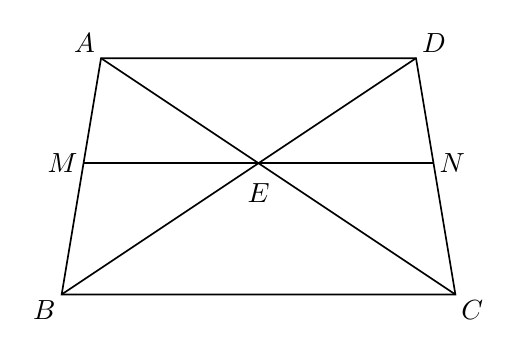
\begin{tikzpicture}[x=1cm,y=1cm,font=\normalsize,
 geometry edge/.style={solid,line width=.6pt},
 geometry mark/.style={solid,line width=.6pt},
 geometry label/.style={font=\normalsize,inner sep=2pt}]
\coordinate (A) at (0.5,3);
\coordinate (D) at (4.5,3);
\coordinate (B) at (0,0);
\coordinate (C) at (5,0);
\coordinate (E) at (2.5,1.6667);
\coordinate (M) at (0.2778,1.6667);
\coordinate (N) at (4.7222,1.6667);
\draw[geometry edge] (A)--(B)--(C)--(D)--cycle;
\draw[geometry edge] (A)--(C);
\draw[geometry edge] (B)--(D);
\draw[geometry edge] (M)--(N);
\node[geometry label,above left] at (A) {$A$};
\node[geometry label,above right] at (D) {$D$};
\node[geometry label,below left] at (B) {$B$};
\node[geometry label,below right] at (C) {$C$};
\node[geometry label,left] at (M) {$M$};
\node[geometry label,right] at (N) {$N$};
\node[geometry label,below=5pt] at (E) {$E$};
\end{tikzpicture}
